\documentclass[12pt]{article}
\usepackage{times} 			% use Times New Roman font

\usepackage[margin=1in]{geometry}   % sets 1 inch margins on all sides
\usepackage{hyperref}               % for URL formatting
\usepackage[pdftex]{graphicx}       % So includegraphics will work
\setlength{\parskip}{1em}           % skip 1em between paragraphs
\usepackage{indentfirst}            % indent the first line of each paragraph
\usepackage{datetime}
\usepackage[small, bf]{caption}
\usepackage{listings}               % for code listings
\usepackage{xcolor}                 % for styling code
\usepackage{multirow}

%New colors defined below
\definecolor{backcolour}{RGB}{246, 246, 246}   % 0xF6, 0xF6, 0xF6
\definecolor{codegreen}{RGB}{16, 124, 2}       % 0x10, 0x7C, 0x02
\definecolor{codepurple}{RGB}{170, 0, 217}     % 0xAA, 0x00, 0xD9
\definecolor{codered}{RGB}{154, 0, 18}         % 0x9A, 0x00, 0x12

%Code listing style named "gcolabstyle" - matches Google Colab
\lstdefinestyle{gcolabstyle}{
  basicstyle=\ttfamily\small,
  backgroundcolor=\color{backcolour},   
  commentstyle=\itshape\color{codegreen},
  keywordstyle=\color{codepurple},
  stringstyle=\color{codered},
  numberstyle=\ttfamily\footnotesize\color{darkgray}, 
  breakatwhitespace=false,         
  breaklines=true,                 
  captionpos=b,                    
  keepspaces=true,                 
  numbers=left,                    
  numbersep=5pt,                  
  showspaces=false,                
  showstringspaces=false,
  showtabs=false,                  
  tabsize=2
}

\lstset{style=gcolabstyle}      %set gcolabstyle code listing

% to make long URIs break nicely
\makeatletter
\g@addto@macro{\UrlBreaks}{\UrlOrds}
\makeatother

% for fancy page headings
\usepackage{fancyhdr}
\setlength{\headheight}{13.6pt} % to remove fancyhdr warning
\pagestyle{fancy}
\fancyhf{}
\rhead{\small \thepage}
\lhead{\small HW8, Bartels}  % EDIT THIS, REPLACE # with HW number
\chead{\small CS 432, Fall 2020} 

%-------------------------------------------------------------------------
\begin{document}

\begin{centering}
{\large\textbf{HW8 - Clustering}}\\ % EDIT THIS
                                % REPLACE # with HW num and ADD title
Logan Bartels\\                     % EDIT THIS
December 6, 2020\\                      % EDIT THIS
\end{centering}

%-------------------------------------------------------------------------

% The * after \section just says to not number the sections

\section*{Q1}

\subsection*{Answer}
\lstinputlisting[language=Python, caption=Python script used to download tweets from 100 accounts listed in 100screen\_names.txt, label=lst:download]{downloadTWeets.py}

\lstinputlisting[language=sh, caption=Shell script used to count usernames in tweets.json and gauge number of tweets., label=lst:checkTweets]{checkNumberOfTweets.sh}

\subsection*{Discussion}
The script in listing \ref{lst:download} is what was used to download tweets for 100 popular Twitter accounts.  Before line 10 you have your basic Twitter authentication for Python.  Line 10 reads in my list of 100 popular twitter accounts stored in ``100screen\_Names.txt.''  It then creates an empty list to store the tweets in.  The for loop starting on line 14 reads ``100screen\_names.txt'' line-by-line.  Because I typed the list manually, with one screen name on each line, I have to get rid of the newline character that is read in with the screen name on line 16.  Then for each username, their 200 most recent English-language tweets (excluding retweets and replies) are downloaded.  Then for each individual tweet, a blank dictionary is created.  The username of the account that made the tweet, the tweet id, and the full tweet text (accessed by setting tweet\_mode to extended) are saved to the dictionary with an appropriately named key for each attribute.  The dictionary is then appended to the empty list created on line 12.  The try-except block is to prevent the script from stopping when a ``page does not exist'' error is encountered.  The list is then dumped to stdout and directed to ``tweets.json''.

The script in listing \ref{lst:checkTweets} performs a grep -c for each account name in ``100screen\_names.txt'' on ``tweets.json''  This is to give me an idea of how many tweets were collected for each account.  The results were not entirely accurate, however.  The inaccuracies are due to some accounts mentioning other accounts, but the mentions were infrequent enough to be negligible.  But I did have to re-select about 50 accounts because that many accounts on my first run produced less than 100 tweets that met my criteria according to the shell script.


\section*{Q2}

\subsection*{Answer}

\lstinputlisting[language=Python, caption=Python script to filter the text of all tweets. Output directed to filteredTweets.json., label=lst:filter]{filterTweets.py}

\lstinputlisting[language=Python, caption=Python script to split the text of each account's tweets into a list., label=lst:gather]{gatherTerms.py}

\lstinputlisting[language=Python, caption=Python script that gets the 1000 most popular words across all accounts., label=lst:count]{countTerms.py}

\lstinputlisting[language=Python, caption=Python script that checks the 1000 most popular words against each account's list of terms and produces a count of how many times each of the 1000 popular words appeared their tweets., label=lst:pair]{pairTerms.py}

\lstinputlisting[language=Python, caption=Python script to construct the account-term matrix., label=lst:makeMatrix]{makeMatrix.py}

\subsection*{Discussion}
Starting with script in listing \ref{lst:filter}, this script reads in ``tweets.json'' and filters each tweet's text to match the requirements for question 2.  To break it down further, the list in ``tweets.json'' is stored in the ``data'' variable on line 7.  Lines 8-12 have variables that store the regular expressions to be run against each term, with each variable being appropriately named to match its regular expression.  Before I go further, I should state that the intent of this script is to create a 1:1 replica of ``tweets.json,'' just with the text filtered to be rid of uris, account names, punctuation, etc.  So similar to listing \ref{lst:download}, an empty list is created to store each tweet.  Then for each tweet dictionary in ``data,'' an empty dictionary is created to store each tweet's attributes as in listing \ref{lst:download}.  Only this time, the username and tweet id of each tweet is immediately stored since I do not have to parse them.  Then the tweet text is stored in ``text.''  After that, the ``re.sub'' function is used to get rid of any terms that match the regular expression passed in as the first parameter on lines 22 and 23.  The second parameter (what to substitute each match with) is the empty string.  The third parameter is the text that is passed in to be run against the regular expression in the first parameter.  The text is entirely converted into lowercase on line 24.  Then, to prepare the text to have any words with non-ASCII characters removed, the text is split into a list, with each element being a term in the text.  For each term in the split text, if it contains a non-ASCII character, remove the term.  I should note that this method does not remove all terms with non-ASCII characters because not all non-ASCII characters presented themselves as something like ``-backslash-u2019.''  For example: after filtering, I noticed a ``youll'' in one of the texts.  Looking at the unfiltered version, it was listed as ``you'll'' instead of ''you-backslash-u2019ll'' (I couldn't get latex to print the backslash).  After the non-ASCII terms are removed, the text is rejoined using the ``join'' function.  From there, just like lines 22 and 23, ``re.sub'' is used to remove matches of the regular expressions passed in.  After filtering is complete, the text is added as a value to the dictionary created on line 17.  The dictionry is then appended to the ``tweet\_data'' list.  The ``tweet\_data'' list is then dumped to stdout using ``json.dump.''  The output was directed to ``filteredTweets.json.''

Moving on to listing \ref{lst:gather}.  This script's purpose is to create a dictionary, with each account being the key and a list of every term in the accounts tweets being the value.  The script reads in ``filteredTweets.json'' and stores that list of dictionaries in ``data.''  An empty dictionary, ``accounts'' is created.  Then the username of every tweet in ``data'' is added as the key in the ``accounts'' dictionary.  The nature of dictionaries ensures that there are no duplicate account names.  The value for each account name in the ``accounts'' dictionary is initially made an empty list.  Lines 13-16 are just a test to confirm I could properly add terms to the values of ``accounts.''  For each account in ``accounts,'' and for each tweet in ``data,'' if the account matches the username in the tweet, then get the text and split it into a list of words.  Then for each word in the split text, append the word to the list of the account's value in ``accounts.''  The result is a dictionary with the account names as keys, and a list of all the terms from that user's tweets.  The ``accounts'' dictionary is dumped using ``json.dump'' to stdout, with the output being directed to ``accountsAndTerms.json.''

Next is listing \ref{lst:count}.  This script is probably the most complex in this report.  It ends up getting the 1000 most popular terms across all accounts.  Let's break down how it gets there.  It starts by reading in ``accountsAndTerms.json,'' and being stored in ``data'' once again.  Two empty dictionaries are created: ``wordCount'' and ``wordList.''  The ``wordCount'' dictionary ends up representing the number of accounts each term appears in, with the terms being the keys, and the number of accounts the term appears in being the values.  The script builds ``wordCount'' by iterating through ``data.values'' starting on line 11.  Recall that data.values is a list of terms, and that ``terms'' is a single list of terms.  The script also iterates through each term in ``terms.''  Then each term is added as a key in ``wordCount,'' with its value being declared an empty string.  The next loop starting on line 15 iterates through each term in ``wordCount.''  A countning variable named ``count'' is declared and initialized to 0 at the start of every iteration.  Then it iterates through each term list in ``data.values'' and checks if the term is in the term list.  If it is, increment the counter, if not, skip to the next term list.  After every term list has be parsed, pass in the final value of the ``count'' variable as the term's value.  The resulting ``wordCount'' dictionary can be viewed in ``termCounts.json.''  That file was created by dumping ``wordCount'' to stdout, and directing the output to it on line 41.  This was done before the rest of the script was written.  The next two loops deal with building the ``wordList'' dictionary.  The first loop, starting on line 24, iterates through the now-built ``wordCount.''  The loop iterates through both ``wordCount's'' keys and values: ``word'' and ``accountCount, '' respectively.  All this loop does is fake the removal of stopwords by only adding the word as a key to ``wordList'' if it appears in more than ten percent and less than fifty percent of all 100 accounts.  The key's value is initialized to an empty string.  The next loop (starting on line 29) starts by iterating through the keys (words) of ``wordList.''  Similar to line 16, a counting variable, ``apperanceCount,'' is initialized to 0 at the start of each iteration.  Then for each list of words in ``data.values,'' if the word is in the list of words, then increment ``appearanceCount'' by adding its current value to the count of that word in the list of words.  If the word isn't in the list of words, skip to the next list of words.  This method ensures that the total number of appearances of the term across all 100 accounts is counted correctly.  After all the lists of words have been parsed, assign the final value of ``appearanceCount'' to the value of the word.  The ``wordList'' dictionary can be viewed in ``wordList.json.''  That file was created by dumping ``wordList'' to stdout and directing the output to that file on line 41 (just replace ``wordCount'' with ``wordList'').  This was done before line 38 was written.  If you compare ``wordList.json'' and ``termCounts.json,'' you will notice that the counts for each word are higher in ``wordList.json'' than ``termCounts.json.''  This is supposed to be the case, as ``termCounts'' only counts the number of accounts each term appears in, versus ``wordList'' that counts the word's appearances over all accounts.  The 1000 most popular words are gotten by sorting ``wordList'' by value in descending order on line 38.  The sorted dictionary, now a nested list, is stored in ``popularWords.''  Each item in the list contains a list with 2 values: a term, and that term's count.  Then the first 1000 items are dumped to stdout on line 40, with the output being directed to ``1000popularWords.json''

Now we have to track how many times each popular word appears in each user's tweets.  This is done using the script in listing \ref{lst:pair}.  This time 2 json files are opened: ``accountsAndTerms.json'' and ``1000popularWords.json.'' They are stored in ``accounts'' and ``terms,'' respectively.  An empty dictionary, ``accountsPopularWords'' is created.  Then there is a function that takes an account name and a term.  It takes that term and finds the count of how many times that term appears in an account's term list, and stores the term and its count in a tuple.  That tuple is stored in ``wordAndCount,'' and returned.  The first loop iterates through the accounts, and assigning each account as the key in the dictionary created on line 10.  The key's value is initialized to an empty list.  The next loop iterates through the new dictionary and each item in ``terms.''  The function on line 12 is called, and the account and term (not the term's count, note the index of the passed in parameter) are passed in.  The returned value is stored in ``wordWithCount.''  Then that variable is appended to the value of the ``account'' key in the ``accountsPopularWords'' dictionary.  This dictionary is then dumped to stdout, with the output being directed to ``accountsAndPopularTerms.json.''  This file contains a dictionary, with the accounts being the keys, and a nested list of terms and their number of appearances in that account's tweets as the values.

Now it's time to build the account-term matrix.  This is done using the script in listing \ref{lst:makeMatrix}.  Two files are opened: ``accountsAndPopularTerms.json'' and ``1000popularWords.json.''  The files are stored in ``accountsPopularWords'' and ``popularWords,'' respectively.  Since this script will write to a csv file, a ``headers'' list is created with only one item: ``Blog.''  This list will serve as the first row in the account-term matrix, which is modeled after blogdata.txt (minus the tab delimiter).  To build the ``headers'' list, the script iterates through the ``popularWords'' nested list, and appends each word to the ``headers'' list.  Lines 15-19 were a test to build subsequent rows of the csv file.  Those rows consist of an account, and its counts for each term.  Now the script is ready to write to ``accountTermMatrix.csv.''  We start by writing the headers to the first row.  Then the loop starting on line 24 iterates through each account and its list of terms.  At the begining of every iteration an empty list called ``row'' is created, and the account name is the first thing added to it.  Then for each term in the list of terms, append the term's count (once again, note the index).  Once all the counts are added, write the row to the csv file.  One thing of note about the csv file is I wrote it with a comma delimiter instead of a tab delimiter like blogdata.txt.  Line 31 can be disregarded.  It was a method of testing to make sure I was correctly reading in files.

\section*{Note}
Questions 3-5 were completed using a copy of the week 12 Google Colab notebook.  The modifications made to it include, and \emph{are} limited to the following:
\begin{itemize}
    \item Eliminated the tab delimiter in the readfile function.
    \item Changed the file in the call to readfile (blogdata.txt) to accountTermMatrix.csv.
    \item Additional cells to output blognames in kclusters were added under the ``kmeans'' section.
\end{itemize}

The notebook can be accessed from the repository and here: \url{https://colab.research.google.com/drive/118JsEQwzDPXRJAde7Tavzk9dDvXgUBIf?usp=sharing}

\section*{Q3}

\subsection*{Answer}
Figure \ref{fig:dendrogram} is on page 19.


\begin{figure}[h]
    \centering
    % trim and clip are used to crop the image, trim=left bottom right top
    % width sets max width, height will be scaled appropriately
    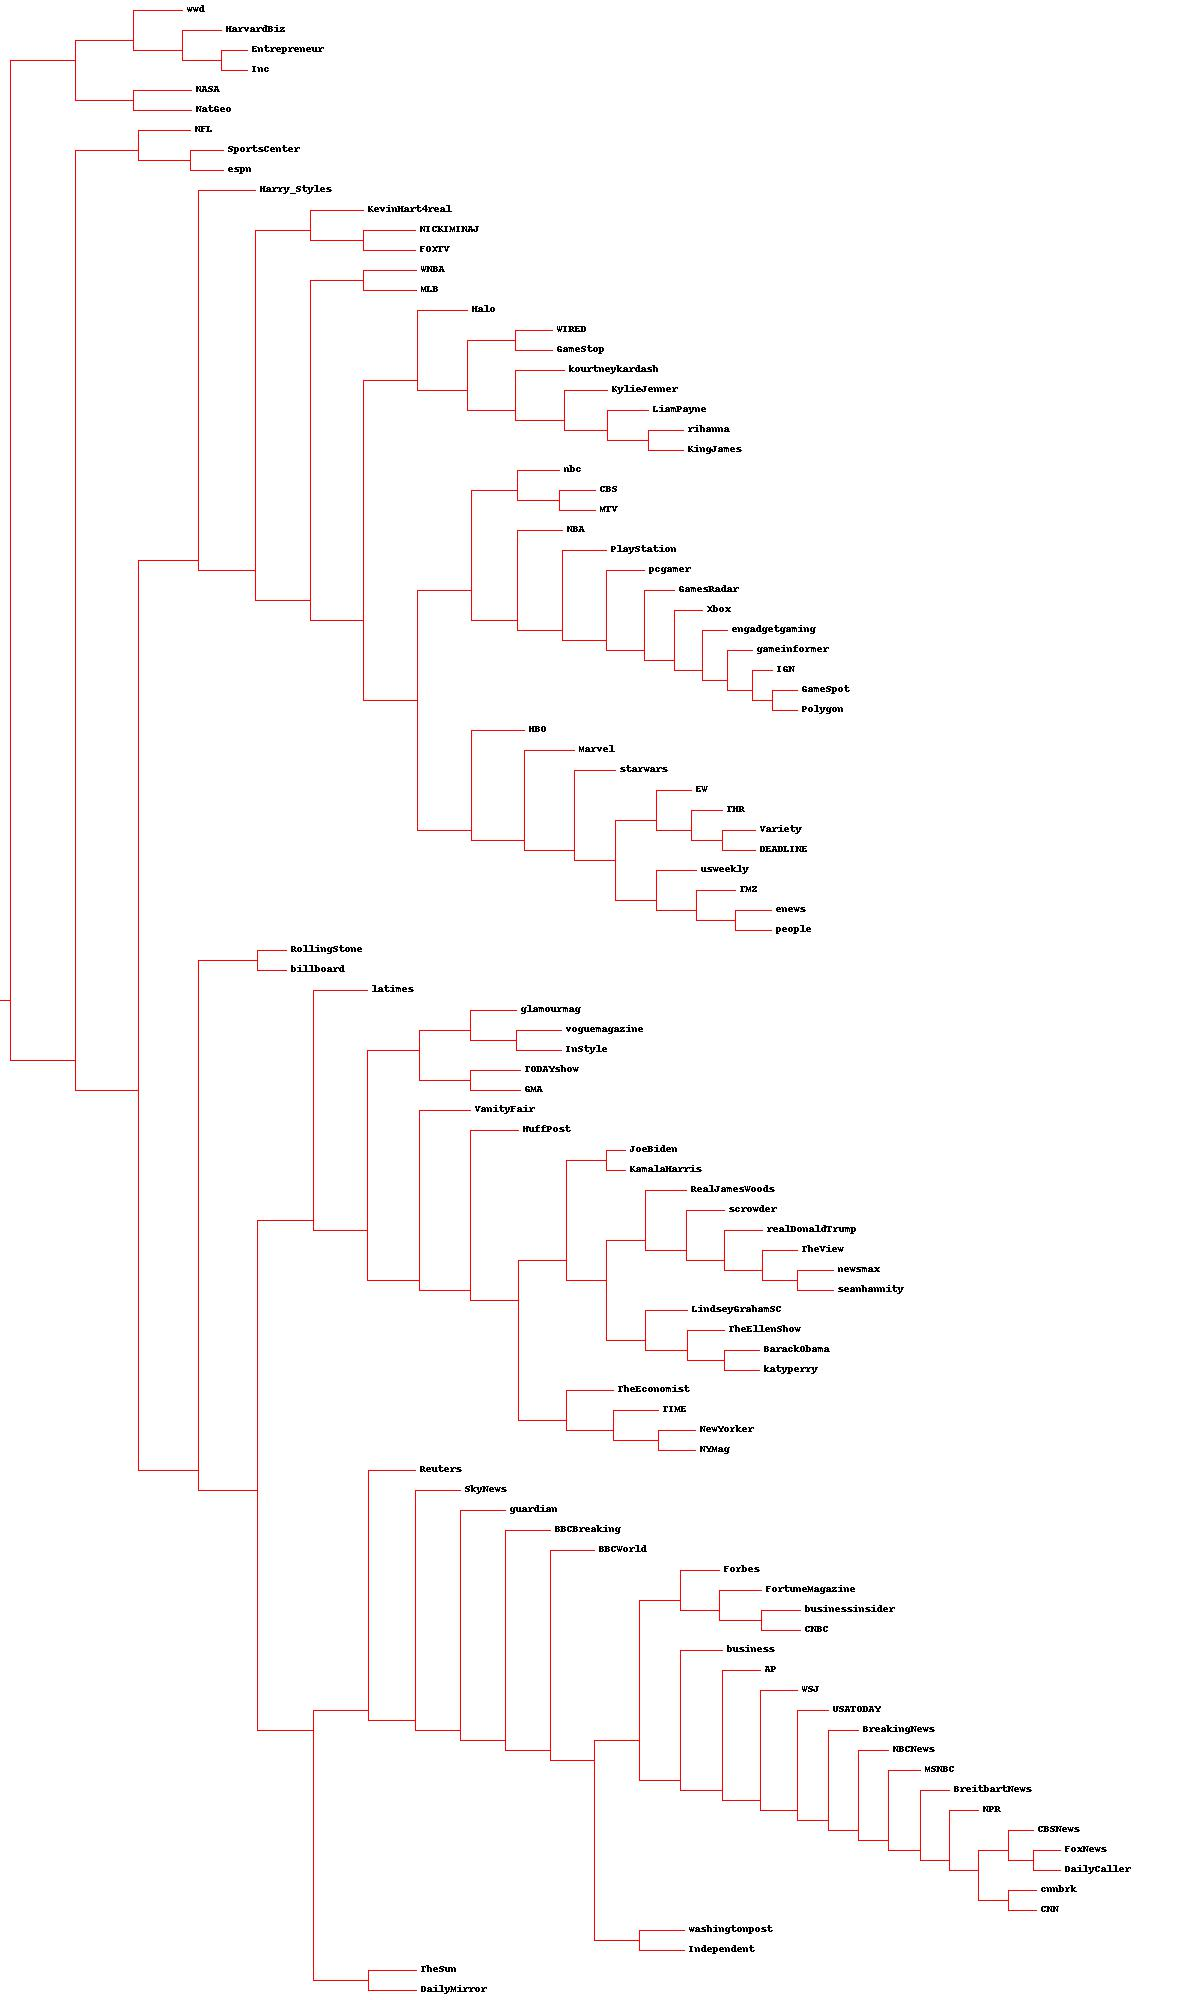
\includegraphics[trim=0 0 0 0, clip, width=0.8\textwidth] {blogclust.jpg}
    \caption{Hierarchical clustering dendrogram.}
    \label{fig:dendrogram}
\end{figure}


\subsection*{Discussion}
The dendrogram shown in figure \ref{fig:dendrogram} is accurate for the most part in its clustering.  Many gaming accounts are clustered together such as PlayStation, pcgamer, gamesradar, Xbox, endgadgetgaming, gameinformer, IGN, GameSpot, and Polygon.  Although there are a couple of outliers in Halo and GameStop being clustered with celebrities.  Many political accounts are also clustered together such as JoeBiden, KamalaHarris, RealJamesWoods(he's very political these days), scrowder, and realDonaldTrump.  There are also many news outlets clustered at the bottom of the dendrogram.


\section*{Q4}

\subsection*{Answer}
\lstinputlisting[caption=Text file with the number of iterations for each value of k, label=lst:iterations]{kMeansIterations.txt}

\lstinputlisting[caption=List of accounts in clusters for k equal to 5., label=lst:k5]{k5Clusters.txt}

\lstinputlisting[caption=List of accounts in clusters for k equal to 10., label=lst:k10]{k10Clusters.txt}

\lstinputlisting[caption=List of accounts in clusters for k equal to 20., label=lst:k20]{k20Clusters.txt}


\subsection*{Discussion}

For the clusters in listing \ref{lst:k5}, I think I can characterize the accounts in each cluster.  Cluster 1 has celebrities and general entertainment.  Cluster 2 has mostly gaming accounts, with some outliers in SportsCenter, KylieJenner, NBA, and NFL.  Cluster 3 has mostly political figures and news outlets.  Cluster 4 is a combination of celebrities and political figures.  Cluster 5 is mostly science, minus DailyMirror.

For listing \ref{lst:k10}, Cluster 1 is mostly sports with 2 outliers in PlayStation and CBS.  Cluster 2 is news outlets.  I cannot characterize Cluster 3.  Cluster 4 is celebrities and general entertainment.  Cluster 5 is mostly celebrities.  Cluster 6 has publishers, 2 of which (HBO and Marvel) are film publishers.  I cannot characterize cluster 7.  Cluster 8 is mostly gaming.  Cluster 9 is political figures and news outlets.  I'm not sure what to make of cluster 10.

For listing \ref{lst:k20}, I'm only going to talk about the clusters I can categorize. If I don't mention one, then either I don't know what to make of it, or it only has 1 account.  Cluster 1 is news outlets.  Cluster 2 is business.  Cluster 3 is more news, as is Cluster 4.  Cluster 5 is entertainment.  Cluster 6 is more news.  Cluster 8 is celebrities.  Cluster 9 is sports.  Cluster 10 is mostly magazines.  Cluster 15 is more news, as is 16.  Custer 17 is gaming.  Cluster 19 is mostly celebrities.  Cluster 20 is a mixture of celebrities and political figures.

I would say that the k value that created the most reasonable clusters is k equals 5.  I feel like those clusters are the easiest to label with a small amount of outliers.

\section*{Q5}

\subsection*{Answer}

Figure \ref{fig:mds} is on page 20.

\begin{figure}[h]
    \centering
    % trim and clip are used to crop the image, trim=left bottom right top
    % width sets max width, height will be scaled appropriately
    
\includegraphics[trim=0 0 0 0, clip, width=0.8\textwidth] {blogs2d.jpg}
    \caption{Multidimensional scaling plot.}
    \label{fig:mds}
\end{figure}

\subsection*{Discussion}
333 iterations were required.  I determined this by running the following cell in the notebook, copy-pasting the outptut into ``MDSIIterations.txt,'' and counting the number of lines.
\begin{itemize}
    \item coords = scaledown(data)
\end{itemize}
I would say the graph shown in figure \ref{fig:mds} is very accurate in its clustering. All the gaming accounts are clustered.  All of the news outlets are clustered together, as well as celebrities and political figures.  I think this plot is more accurate than the dendrogram.



\section*{References}


\begin{itemize}
    \item {Parse Twitter Hashtags, Usernames \& URLs with JS, \url{https://www.benmarshall.me/parse-twitter-hashtags/}}
    \item {Best Practice to Extract and Remove URLs from Python String – Python Tutorial, \url{https://www.tutorialexample.com/best-practice-to-extract-and-remove-urls-from-python-string-python-tutorial/}}
    \item {The Perfect URL Regular Expression, \url{https://urlregex.com/}}
    \item {Read JSON file using Python, \url{https://www.geeksforgeeks.org/read-json-file-using-python/}}
    \item {Python | Remove punctuation from string, \url{https://www.geeksforgeeks.org/python-remove-punctuation-from-string/}}
    \item {Python: Remove words from a string of length between 1 and a given number, \url{https://www.w3resource.com/python-exercises/re/python-re-exercise-49.php}}
    \item {Lowercase in Python, \url{https://www.educba.com/lowercase-in-python/}}
    \item {Python String encode() Method, \url{https://www.w3schools.com/python/ref_string_encode.asp}}
    \item {Python 3 - String decode() Method, \url{https://www.tutorialspoint.com/python3/string_decode.htm}}
    \item {Python String split() Method, \url{https://www.w3schools.com/python/ref_string_split.asp}}
    \item {Python String join() Method, \url{https://www.w3schools.com/python/ref_string_join.asp}}
    \item {Week 12 Colab Notebook \url{https://colab.research.google.com/github/cs432-websci-fall20/assignments/blob/master/432_PCI_Ch03.ipynb}}
    \item {Week 12 Slides, \url{https://docs.google.com/presentation/d/1Sz5tSqXBjMCLOIq7oIEq53BXDfLvNWwjIZFug3Z_aVE/edit?usp=sharing}}
\end{itemize}

\end{document}

